\documentclass[12pt]{article}
\usepackage{tikz}
\usetikzlibrary{arrows,positioning}
\begin{document}
	

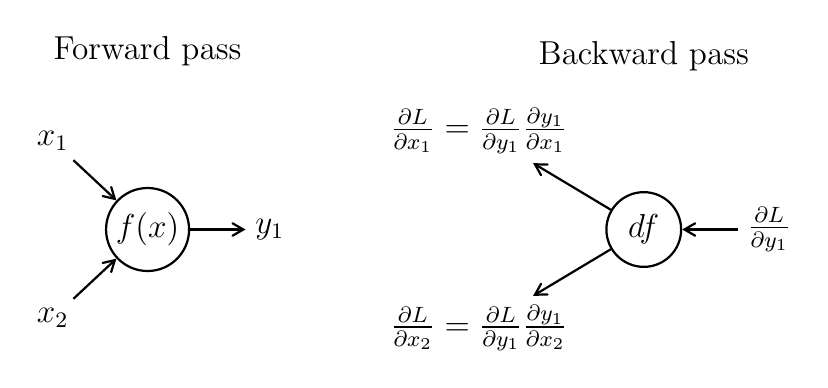
\begin{tikzpicture}[arrow/.style={thick, >=angle 60}]
	\node[draw, circle,thick,minimum width=3em, inner sep=0] (fp) {\large $f(x)$};
	\node[above left = 2em of fp] (x1) {\large $x_1$};
	\node[below left = 2em of fp] (x2) {\large $x_2$};
	\node[right = 2em of fp] (y1) {\large $y_1$};
	
	\node[above = 4em of fp] {\large Forward pass};
	
	\draw[->,arrow] (x1) -- (fp);
	\draw[->,arrow] (x2) -- (fp);
	\draw[->,arrow] (fp) -- (y1);

\node[draw, circle,thick,minimum width=2.7em, inner sep=0, right = 15 em of fp] (bp) {\large $df$};
\node[above left = 2em of bp] (bx1) {\large $\frac{\partial L}{\partial x_1}=\frac{\partial L}{\partial y_1}\frac{\partial y_1}{\partial x_1}$};

\node[below left = 2em of bp] (bx2) {\large $\frac{\partial L}{\partial x_2}=\frac{\partial L}{\partial y_1}\frac{\partial y_1}{\partial x_2}$};

\node[right = 2em of bp] (by1) {\large $\frac{\partial L}{\partial y_1}$};

\node[above = 4em of bp] {\large Backward pass};

\draw[<-,arrow] (bx1) -- (bp);
\draw[<-,arrow] (bx2) -- (bp);
\draw[<-,arrow] (bp) -- (by1);
\end{tikzpicture}
	
\end{document}